%%%%%%%%%%%%%%%%%%%%%%%%%%%%%%%%%%%%%%%%%%%%%%%%%%%%%%%%%%%%%%%%%%%%%%%%%

% Definitions
%\pagestyle{empty}
\documentclass[12pt,preprint]{aastex}
%\documentstyle[emulateapj,danonecolfloat]{article}
%\usepackage{emulateapj,danonecolfloat}
\usepackage{rotating}

%------------------------------------------------------------------------------
% DEFINITIONS
%------------------------------------------------------------------------------
%
% Equations:
%
\def\BE{\begin{equation}}
\def\BEL#1{\begin{equation}\label{#1}}
\def\EE{\end{equation}}
%
% Random stuff:
%
\newcommand{\etal}{{\it et al.}~}
\newcommand{\LOGTEN}{{\log_{10}}}
%
% Units (math mode)
%
\newcommand{\Ang}{{\rm ~\AA}}
\newcommand{\cm}{{\rm ~cm}}
\newcommand{\dfdegree}{^\circ}
\newcommand{\degree}{^\circ}
\newcommand{\ergs}{{\rm ~erg~s}^{-1}}
\newcommand{\ergscmang}{{\rm ~erg~s}^{-1}{\rm cm}^{-2}{\rm\AA}^{-1}}
\newcommand{\ergcmHzsr}{{\rm ~erg~cm}^{-2}{\rm s}^{-1}
            {\rm Hz}^{-1}{\rm sr}^{-1}}
\newcommand{\Jy}{{\rm ~Jy}}
\newcommand{\JypSr}{{\rm ~Jy~sr^{-1}}}
\newcommand{\GHz}{{\rm ~GHz}}
\newcommand{\Hz}{{\rm ~Hz}}
\newcommand{\K}{{\rm ~K}}
\newcommand{\kms}{{\rm ~km/s}}
\newcommand{\MAG}{{\rm ~mag}}
\newcommand{\microK}{\mu{\rm K}}
\newcommand{\MJy}{{\rm ~MJy}}
\newcommand{\mJy}{{\rm ~mJy}}
\newcommand{\MJypSr}{{\rm ~MJy~sr^{-1}}}
\newcommand{\nWpMMSr}{{\rm ~nW~m}^{-2}{\rm sr}^{-1}}
\newcommand{\mK}{\rm ~mK}
\newcommand{\mm}{{\rm ~mm}}
\newcommand{\nMgy}{{\rm nMgy}}
\newcommand{\pc}{{\rm ~pc}}
\newcommand{\pix}{{\rm ~pix}}
\newcommand{\s}{{\rm ~s}}

%------------------------------------------------------------------------------
% TITLE PAGE
%------------------------------------------------------------------------------

\begin{document}

\title{The Sloan Digital Sky Survey Spectroscopic Reduction Pipeline}

\author{
S. Burles\altaffilmark{\ref{MIT}}
and D. J. Schlegel\altaffilmark{\ref{Princeton}}
}
\altaffiltext{1}{Department of Physics and Kavli Institute for Astrophysics 
and Space Research, MIT, Cambridge, MA 02139 \label{MIT}}
\altaffiltext{2}{Princeton University Observatory, Peyton Hall, Princeton,
NJ 08544 \label{Princeton}}

%------------------------------------------------------------------------------
% ABSTRACT
%------------------------------------------------------------------------------

\begin{abstract}
The Sloan Digital Sky Survey (SDSS) fiber-fed spectrographs have been used
to obtain spectra for ~$600,000$ galaxies, quasars and stars
with a resolution of ~2000 over the wavelength range 3800\AA -9600\AA.
We present the algorithms for reducing the raw data to
wavelength-calibrated, flux-calibrated one-dimensional spectra.
The wavelength calibration is shown to have an accuracy of $3 \kms$,
and the broad-band spectrophotometry to have an accuracy of better than $6\%$.

%------------------------------------------------------------------------------
% SUBJECT HEADINGS
%------------------------------------------------------------------------------
\emph{Subject headings: }
instrumentation: spectrographs --- techniques: spectroscopic --- 
methods: data analysis --- surveys -- galaxies: distances and redshifts
\end{abstract}

%------------------------------------------------------------------------------
% INTRODUCTION
%------------------------------------------------------------------------------
\section{INTRODUCTION}
\label{sec_intro}
The Sloan Digital Sky Survey (SDSS) is a 5-band photometric survey of
approximately $10,000$ square degrees of the Northern sky and a concurrent
redshift survey of up to a million galaxies and 100,000 quasars
selected from the imaging survey (York et al 2000).  The primary 
science goals of the project are to provide the data to investigate the
large scale structure of the Universe and other extragalactic science.

In this paper, we describe the details of the SDSS 2-d spectroscopic pipeline
(idlspec2d) including steps starting with processing of the raw CCD frames 
to final flux calibration and spectral co-addition.  Downstream pipelines 
which calculate redshifts, spectral types, emission and absorption line 
identification, and velocity dispersions are described elsewhere.
As of writing the 2-d pipeline has been run successfully on all spectroscopic
data obtained in the course of the survey from February 28, 2000 
(Modified Julian Data, MJD 2451602) 
to June 15, 2005 (MJD 2453536).  Over this timespan, which includes public data 
releases EDR through DR5 (Stoughton et al 2002, 
Abazajian et al 2003, 2004, 2005, Adelman-McCarthy et al 2006)
, SDSS obtained survey quality spectroscopic data on
1656 fiber pluggings (640 fibers each in 1575 unique plates).   
A total of 972,111 sky positions were targetted, with the following 
breakdown in the best matched spectral classification:  651920 galaxies, 
208054 stars, 112137 QSOs and 51300 sky spectra.

Mean exposure time per plate is 3914 seconds, and the median is 3302 seconds.
;
;   Should we include a histogram of exposure times??
;

In Figure 1 we show three of the data quality diagnostics. This figure shows
the effective signal-to-noise ratio of each spectroscopic plug plate 
normalized to 3600 seconds exposure time, the median seeing in arcseconds,
and the RMS guide probe offset
in arcseconds, versus time in days after Feb 26, 2000 (MJD 2451600).

The data reduction and products described herein are very similar to
those produced by the official SDSS data releases, 
with the most significant differences begin in our treatment of 
spectro-photometric calibrations.  The data as processed as described
are released
with this paper and may be accessed via the WWW.\footnote{Full details
are at \texttt{http://spectro.princeton.edu}}
Future data releases will also be accessible at this site. 

%------------------------------------------------------------------------------
%------------------------------------------------------------------------------
\section{SDSS SPECTROGRAPHS}
\label{sec_spectrographs}

The SDSS spectroscopic survey was carried out with twin multi-fiber 
double spectrographs mounted at the back of the SDSS telescope 
(see Gunn et al.  2006).  
One of nine spectrograph cartidges can be mounted for a single
spectroscopic observing sequence.  The cartridge holds a single aluminum
plate, 813mm in diameter, pre-drilled and plugged with 640 fibers 
fed into the twin spectrographs, 
and 11 coherent fibers fed into a simple air-cooled camera (model \#??)
for telescope guiding.

The fibers are 180 $\mu m$ in diameter and subtend $2.97"$ at Cassegrain focus.
The fibers accept the f/5 beam directly and, due to focal degradation, input
an f/4 exit beam into each of the spectrographs.  The fibers are mounted in
bundles of 20 with inter-fiber spacings of 390 $\mu m$.  Sixteen bundles are
mounted on a single slithead with a radius of curvature of 640 mm and have
an extra spacing of approximately 200 $\mu m$ between bundles.

In Figure 1, we show a top-view schematic of one the spectrographs.  Here
we provide a short summary of the light path starting at the slithead,
further details can be found in Uomoto et al. (20??) and Gunn et al. (2006).
The output light from the fiber is collimated by a spherical mirror
(of radius of curvature 1264 mm), which is aligned by 3 motor mounts to
control focus, tip and tilt.  A left/right Hartmann mask 
covers the collimator to act as both a spectrograph shutter and traditional 
Shack-Hartmann mask for focus tests.  The collimator in spectrograph 2
was coated with an enhanced silver coating and delivers slightly higher
reflectivity compared to the aluminum coated collimator in spectrograph 1.
The collimated beam encounters a 40mm thick dichroic (beamsplitter) which
reflects light blueward of 6000\AA.  The blue reflected light is dispersed
with a 640 l/mm grism with zero deviation at 4960\AA.  The red transmitted
light is dispersed with a 440 l/mm grism with zero deviation at 7400\AA.
The dispersed light in each arm of the spectrograph enters a transmission camera
with a 240mm focal length (demagnification of 2.5) which is tuned for the 
corresponding range of wavelengths.  Each of the 4 cameras produce RMS 
spot sizes of approximately 20$\mu m$ over a 16.5$\degree$ diameter 
field-of-view delivered to a single thinned Tektronix 2048x2048x24$\mu m$ CCD
(see Gunn et al. 2006).
An external focus ring is adjustable by hand for each CCD camera to accomodate
differential focus changes not corrected with the common collimator.
The four spectrograph cameras are labeled $``$b1, r1, b2, r2", where
1 and 2 refer to the spectrographs and b and r to their blue and red sides.  


\section{Typical Spectroscopic Observations}
\label{sec_observ}

At the beginning of a typical survey night, up to 9 plates have been mounted
in cartridges, plugged with 640 science fibers and 11 guide fibers. 
The positions of the 640 fibers along each of the two fiber slitheads
%are mapped by the 8th wonder of the world,
by 
the SDSS plugplate fiber mapper (Schlegel and Finkbeiner, unpublished).
All usable spectroscopic data obtained for a single plugging, 
and therefore a single fiber mapping, will eventually be combined into 
a final data product for that plugging.  In this scheme, an individual 
output spectrum is uniquely specified by the plate number, the first night
of observations\footnote{On occasion, to accumulate enough signal, a given
plate/plugging configuration may be exposed on more than one night.} (in MJD), 
and the science fiber number.

A plate is mounted in the telescope through a efficient procedure described
by Gunn et al (2006).  The switch from the imaging camera to a spectroscopic
cartridge takes an average of 30 minutes, while a switch from one cartridge
to another takes 10 minutes.  Once the cartridge is mounted, 
the telescope is slewed to the coordinates of the plate center.  
Before acquisition of the guide stars, the 8 flat-field petals are closed and
a sequence of one 10-second flat-field exposure and one 2-second 
Neon-Mercury-Cadmium arc exposure are obtained.  While the arc-lamp frame is
being read out, the flat-field petals are opened, and guide stars are acquired
through the 11 coherent guide bundles (9 are 7$"$ in diameter and 
2 are even larger at 11$"$).
With at least 4 guide stars acquired, closed loop guiding is started, and
usually converges to stable guiding within 2 minutes.
The plate scale of the SDSS telescope can be adjusted, and the guiding software
suggests a scale change if one is required.  Once close loop 
guiding has settled, the first science exposure is started.  The typical 
exposure time is 900 seconds, but exposure times from 600 to 1200 second are
not unexpected based on conditions and time constraints.  A second exposure
is started immediately after the first science exposure is complete and read
out.
A fast Linux workstation onsite copies the data from the data acquisition host,
and automatically performs a quick spectral extraction with a subset of the 
steps explained here.  The results are posted to sos.apo.nmsu.edu, and
the SDSS observers can check the signal-to-noise ratio (S/N) 
obtained in each of the 4 spectroscopic
cameras in real-time.  A plate is considered to have met SDSS survey standards
if all 4 cameras have a cumulative (S/N)$^2 > 15$ at 
fiber magnitudes of 20.33 and 20.06 in SDSS g and i filters respectively.  

\section{IMAGE PROCESSING}
\label{sec_process}

sdssproc:

1000 lines of IDL code...

read opEcalib
     op something else

Read file header, require...
mention spHdrFix here.



\section{SPATIAL TRACING}
\label{sec_tracing}

trace320, Trace crude, and trace fitting


\section{OPTIMAL EXTRACTION}
\label{sec_extract}

We utilize an optimal extraction procedure to transform a 2-dimensional image of
the fiber spectrograms to a set of 320 one-dimensional spectra 
(per spectrograph).  We use the same procedure on all processed frames, 
and will describe the details in processing the flat-field frames, the
arc lamp frames, and finally the science frames.  
The extraction is performed row-by-row, so each frame requires an 
outside loop over 2048 individual rows.
The counts in each row of 2048 columns are modeled with a linear 
combination of 320 profiles plus a low-order
polynomial background.  In addition, deviations to the trace centers and
the profile widths are calculated as linear basis modes (reflecting the first
and second spatial derivatives, respectively).  The compiled routine
we implement to fit the profiles in a single row (extract\_row.c) can
be invoked with any combination of these parameters.  The parameters are
sorted in order of fiber number with background parameters included at the
end of the list.  This facilitates a banded matrix inversion, and 
significantly increases the speed of the Cholesky decomposition step in each
iteration of the extraction.

We decided to perform profile fitting to the 
SDSS spectral images for the following reasons:  

\begin{enumerate}

\item{The fiber profiles overlap significantly with their nearest neighbors.}

\item{The profiles are relatively stable and smoothly vary over 
location on the CCDs.  They result from the convolution of the fiber 
illumination pattern + the point-spread function
of the optics in the SDSS spectrographs + the window funciton of the 
Site CCD 24 micron square pixels. }

\item{A least-squares fit with the true profile delivers an 
unbiased and minimum variance estimate of the counts (e.g. Horne et al. 1995).}

\item{A model profile fit leads to a model image of the SDSS data,
and iteration allows cosmic-ray rejection and goodness-of-fit tests.}

\item{A valid estimate of the error in a flux measurement at 
each spectral pixel can be made.}

\end{enumerate}

The major obstacle to actual optimal extraction is the determination of 
the exact shape and position of the underlying profile.  
We investigated a range of symmetric, analytic profiles with a 
minimum number of free parameters.  In the end, we found the best 
results using a simple Gaussian (noted as PROFTYPE 1 in the primary HDU header) 
or a slightly steeper profile characterized by 
the average of a profile with $e^{-|x|^3/\sigma^3}$ and a Gaussian
with the same sigma (PROFTYPE 3).  The profiles are defined to be 
normalized to unity, so the amplitude of the profile fit is a 
direct estimator of the counts at a single spectral position. 

Extraction is first carried out on all flat-field exposures 
(typically 10 second observations of 4 quartz lamps projected on petals covering the entrance aperture of the telescope) which were observed
with a common plug plate configuration (a spectroscopic sequence). 
The flat-field extraction is used to determine the shape of
the profile as a function of wavelength and position on the CCD.  
The resulting spectral extractions are also used to 
determine the empirical fiber-to-fiber variations in throughput 
as a function of wavelength.   
A flat-field frame is rejected by the pipeline if one of the
following conditions is met:  1) more than 2\% of the CCD pixels are labeled
bad by {\tt sdssproc} (see below), 
2) more than 100 rows of the image have more than 20 saturated pixels, 
3) the 80th percentile count level is less than 1000 counts, 
4) fewer than all 8 flat-field telescope petals were closed, 
5) fewer than all 4 flat-field lamps were on,
6) more than 10000 pixels were rejected during fiber tracing, 
7) fiber tracing fails, or traces are separated by less than 3 pixels anywhere
on the flat-field image.

The first very critical step is to robustly determine the fiber positions 
in CCD pixel coordinates.
This is performed by identifying peaks in a cross-sectional cut across 
the center row (actually a median cross-section of the central 9 rows).  
The correct identification of the 320 fibers per frame can be 
uniquely determined by demanding a wider spacing between the bundles 
of 20 fibers (spaced by about 10 pixels) relative to the nominal inter-fiber 
spacing (6.1 pixels on average).  Once the starting peaks and 
identification have been determined, we trace the fiber centers 
by performing flux-weighted centroids on subsequent rows
using the previous row's center as the intial guess.  This has proven to 
work well on SDSS flat-fields, and we have yet to uncover a failure 
mode in over 10000 flat-field frames.
The flux-weighted centroids do have scatter from shot noise, 
so we fit a 7th order polynomial to each set of fiber centroids, 
and the best-fit coefficients are stored to represent the fiber positions 
on each flat-field frame.


Each flat-field frame is extracted twice, once assuming a Gaussian
profile and again assuming the steeper PROFTYPE 3 profile.  In both cases,
the width is allowed to vary freely.  The total number of free parameters
per row in the flat-field extractions is equal to 2 per fiber plus 10
parameters to represent a smooth polynomial background.  After the extractions
are complete, $\chi^2$ is computed by directly comparing the model fit
to the flat-field image.  The median $\chi^2$ for each case is compared
directly, and the better fit and profile (lower median $\chi^2$) are retained
and implemented for the extraction of the remaining frames.  Also retained
is a smooth polynomial fit to the average profile width in each fiber bundle
as a function of CCD row number.

After all flat-field frames for a given sequence have been extracted
and stored, the arc-lamp frames in the same sequence are extracted.  
Each arc-lamp frame is matched with the nearest (in time) 
non-rejected flat-field frame.  The matched flat-field gives the 
initial trace centers to
be assumed, as well as the profile shape and width determined from the
flat-field.  To account for any flexure between the frames, the trace
centers are allowed to shift/stretch to the arc-lamp image given a 
3x3 polynomial distortion kernel over the entire extent of the image
(match\_trace.pro).

The arc-lamp frames are extracted row-by-row, in the same
manner as the flat-fields, the number of free parameters assumed
for the model fit is 2 per fiber (profile area and width) and 1 parameter
to fit for a constant background per row.  The restricted freedom in the
background parameterization reflects the lower scattered light levels in
the images of the arc-lamps.

\subsection{Wavelength solution}

We determine an initial wavelength solution for every arc-lamp frame
successfully extracted in the following manner:

For the appropriate side of each spectrograph (red or blue), we 
construct a list of suitable unblended lines from a parent list including
known lines of Mercury, Cadmium, Neon and (a trace of) Argon 
that are readily observable in the standard set of SDSS arc-lamps. 
A representative spectrum is calculated as the median extracted spectrum
of the 5 closest $``$unflagged" spectra falling near the central columns 
of the arc-lamp image.  This median arc-spectrum is matched with 
cross-correlation to a simulated spectrum of suitable arc-line positions and 
strengths by systematically searching a small volume of 
parameter space which conservatively covers
the polynomial coefficients of the SDSS wavelength solution.
In the first iteration, we search a set of 
100 coefficient vectors allowing for quadratic changes and return 
the best match.  In the second iteration, we search in a smaller region
about the previous best match, and search a list of 125 coefficient vector
allowing for cubic deviations.  The coefficient vector with the best
match from the second iteration is returned as an initial guess along with
the cross-correlation coefficient.  

We apply the best guess coefficients to predict the approximate pixel 
positions of the suitable list of arc lines.  The arc line centroids
are traced across extracted spectra (along the axis of 320 fibers).
The centroids are fit to a smooth polynomial as a function of fiber
position on the arc-lamp image, and subsequently fit through 6 iterations
with simple flux weighting to arrive at a converged measure of line 
centroids in each extracted spectrum.  Lines are excluded from the resulting
list if the flux-weighted centroids are bad in more than 10\% of the
spectra or if the RMS residuals are larger than 0.2 pixels.
We perform an iterative 4th order Legendre polynomial fit of 
logarithmic wavelength as a function of pixel in each spectrum, 
and retain a list of rejected centroids, 
which have deviations relative to the model of
10\% of a pixel width.  An additional requirement is applied to each
suitable arc line, wherein the line is rejected in no more than 3 fibers
per bundle of 20.  Rejected centroids are replaced with the appropriate
positions based on a linear interpolation of the differences of non-masked
centroids relative to updated polynomial fits per spectrum.
The final set of positions, where the same number of line positions have
reliable centroids per spectrum, are fit with equal weighting per line
position to produce the final wavelength
coefficients which give the logarithmic (base 10) wavelengths as a function
of spectral pixel.

An arc-lamp image is declared unacceptable using the first 4 tests as employed
in tests of the flat-field images.  In addition, an arc-lamp exposure
is declared unacceptable (``BAD") if any of these following criteria are met:
5) not all 8 arc-lamps are on: 4 Neon lamps and 4 Mercury-Cadmium lamps,
6) the initial cross-correlation coefficient is less than 0.5,
7) fewer than 6 arc lines are acceptable after quality assurance checks.

The width of unblended arc lines are determined as an average over
each bundle of 20 spectra.  In short, the arc-lamp emission lines 
are extracted (with a Gaussian spectral profile) 
allowing free parameters for the area and width of each suitable line.
The resulting Gaussian widths per fiber bundle are fit 
with a low order polynomial as a function of average line position
(the fit is quadratic and cubic for the blue and red side respectively).
The fitted quantity is referred to as the arc-lamp dispersion,
but the values reflect the standard deviation of a Gaussian 
profile in pixel units and represents the line-spread function of the 
arc-lamp spectra.  Detailed analysis of the measured arc-line widths
compared to the observed sky emission line shapes show less than a 1\%
difference on average (McDonald et al. 2006). 

%%(or just refer to data model appendix instead of the paragraph below:)
%%
%%The arc-lamp reductions are written to disk at this stage, and
%%stored in an extended FITS file:  HDU \#0 contains the processed
%%and extracted arc-lamp spectra as counts per pixel, HDU \#1 contains
%%the identified arc line wavelengths and the measured line centroids
%%(including replaced positions of rejections), HDU \#2 contains a single
%%structure with the Legendre polynomial coefficients applicable to each
%%of the 320 arc-lamp spectra, HDU \#3 contains the maskbits for each spectrum,
%%and HDU \#4 contains the polynomial coefficients to describe the arc-lamp
%%Gaussian widths as a function of spectral pixel.

\subsection{Constructing fiber flats}

The final step in the reduction of the calibration frames in a given
sequence is the construction of the fiber flat vectors.  Each flat-field
frame is matched to the nearest arc-lamp frame as before, and the
final flat-field fiber spectra are extracted in two steps.  The first
step uses the preferred spatial profile and width determined above,
and the extraction procedure produces a model of the flat-field frame.
The model is used to subtract a diffuse scattered background given
by an exponential point-spread function of :  (CCD halo PSF).
We apply a 1-dimensional version of this 2-d PSF as an approximation,
and allow the PSF to vary appropriately with wavelength.
The final extraction is applied to the scattered light subtracted flat-field
image allowing for 2 free paramters per fiber per row and 
5 background parameters per row.

The final flat-field spectra are stored as 
detected counts per fiber per pixel with wavelengths of each pixel
given by the solution of the matched arc-lamp frame.  
We model the flat-field spectra as the product:


\begin{equation} 
{\rm Model}_{ij} = A \times {\rm SF}(\lambda) \times {\rm (fiber~flat)_i} (\lambda) 
\end{equation} 
where $A$ is a overall normalization in counts, 
$SF$ is the average wavelength dependent response called the ``superflat'', and
${\rm fiber~flat_i}$ is the fiber-to-fiber response as a function of wavelength.
This model of the extracted flat-field spectra provides a transformation to
compare detected counts from one fiber to another.
The flat-field vectors correct the differential response due to the individual fiber
throughput, as well as the small relative differences in the size of the
spectral pixels at a constant wavelength.  

The common normalized response, $SF$, is specified as a B-spline (basis spline)
function with breakpoints spaced at approximately the native pixel spacing.
An example of normalized individual fiber spectra 
and the resulting B-spline fit is shown in Figure 3.  The individual fiber
flat vectors are fits to the ratio of the extracted spectra to the superflat
(defined above).  The individual vector fits are also B-splines with breakpoints
spaced approximately every 5 native pixels.  The final set of flat vectors are
stored as an image with dimensions of Nfiber,Npixels.

\subsection{Object Extraction}

With the extracted calibration frames for a given spectroscopic sequence
reduced, we proceed to extract the remaining science frames.
%To minimize the differences between individual science frames
We first select a set of arc-lamp and flat-field frames as the common
choice of initial calibrations for all science frame extractions in a given
observing sequence.  We loop through the science exposures, processing the
raw images with bias and pixel-to-pixel flat images (see section ??).
We reject a science exposure outright if 1) more than 10\% of the pixels
are flagged as bad, 2) more than 100 rows have more than 20 saturated
pixels, 3) the 25th
percentile count level is greater than 1000 counts (the nominal level
is of order 10 counts), 4) any of the flat-field petals are closed, or 5)
any of the calibration lamps are recorded as on.

Inputs to object extraction include the wavelength coefficients derived
from the associated arc-lamp exposure, both the superflat and fiber flat
vectors from the selected flat-field exposure, the profile shape and width
as a function of position on the CCD image.

The first step in object extraction is a simple tophat aperture (boxcar) 
extraction centered at the fiber positions determined from the flat-field 
and with a full spatial width of 6 CCD pixels.  The median counts per fiber 
are passed directly to a test for overly bright fibers. Fiber spectra are 
identified as bright (a.k.a. $``$WHOPPING") 
if the median counts per pixel in the 
boxcar extraction are greater than 10000 counts above the median in the 
frame.  In addition, only the brightest fiber in a spatially contiguous set of 
bright fibers is labelled $``$WHOPPING".  Each whopping fiber adds an additional
background parameter to the fit per row, which is an exponential profile
with a spatial scale of 25 pixels.  Such a profile correlates with many
neighboring fibers, so the parameter is treated as a background to supplement
the smooth polynomial background.  The flux contained in the exponential 
profile is not included in the extracted spectra.

A pixelmask vector is created for each fiber spectrum to be extracted.
See Appendix B for a description of the mask bits and their use.

We fit for a slight distortion of the stored flat-field fiber traces to 
best match the fiber positions of the science image.  Nominal shifts and
distortions are usually less than a native CCD pixel.  The science frame
is now extracted in a series of 6 steps which we detail below.

\begin{enumerate}
\item{Initial extraction including broad wings of bright (WHOPPING) fibers.}
\item{Reconstruct a smooth background light model based on fitted parameters.}
\item{Calculate a scattered halo image using the model of the fiber spectra less
the aforementioned smooth background.}
\item{Re-extract fiber spectra on the scattered halo subtracted image.}
\item{Reconstruct smooth background and subtract.}
\item{Final extraction with no free parameters in the background and
no free parameters in the profile widths.}
\end{enumerate}

The extracted science spectra are first normalized by the fiber flat vectors.
Strong atmospheric emission lines (sky lines) are identified in the the 
set of spectra, and the wavelength solution is shifted and stretched 
to match the identified sky line positions.  
Examples of the shift corrections are shown in Figure 9.  
The widths of the identified sky lines are also measured with the same method
as the arc-line width measurements.  All spectra are also normalized by
the average flat-field spectrum (the superflat) to remove small scale
features likely attributed to the chromatic response of the dichroic.
The wavelength solution is corrected to both vacuum wavelengths and the
solar system barycenter velocity frame.

\subsection{Sky Subtraction}

Sky subtraction is performed on a frame by frame basis using the 
``flattened'' wavelength calibrated extractions.  The goal of sky subtraction
is to estimate the expected background counts contributing to each of 
the native 320x2048 pixels in each extracted frame.  A ``supersky'' model 
at a fiducial airmass of 1 is constructed by performing iterative fits to
the extracted spectra associated with blank sky positions (so-called
``sky'' fibers).   The following steps are taken in 3 sequential iterations
in order to produce the sky-subtracted spectra:

\begin{enumerate}

\item{Identify the "sky" fibers which have no bits flagged 
in the fiber mask array.}

\item{Divide each sky spectrum by the airmass of the fiber position appropriate
for the midpoint of the observation to produce respresentative sky spectra for 
an airmass of 1.  The inverse variance is scaled accordingly.}

\item{Group and sort the sky spectra as a function of wavelength.  This step
transforms a 2-dimensional set of $N_{\rm sky}$ x 2048 pixels into a sorted 1-dimensional array.  
Each pixel maintains its associated central wavelength and inverse variance. }

\item{Perform a single cubic B-spline fit as a function of wavelength.  
The number of breakpoints (number of free parameters is 4 greater) is set 
at 2048 on the red side and 1536 on the blue side.  The breakpoint spacing 
is set automatically to maintain approximately constant S/N between breakpoint 
positions. The B-spline fit itself is iterative, with upper and lower rejection 
thresholds set to mask bad or deviant pixels. }

\item{The B-spline fit is evaluated at all 320x2048 wavelengths representing all
spectral pixels in the frame.  The airmass correction is applied for each individual 
fiber, and the rescaled super-sky is subtracted from each spectrum.}

\item{Estimate the significance of the residuals in the sky fibers used for the
fit in wavelength bins separated by breakpoints determined above.  For each bin
where the 67th percentile of $\chi^2$ is greater than 1, we rescale 
all the inverse variance values down by the 67th percentile value of $\chi^2$.
The rescaling is actually done with a smooth interpolation as a function of 
redshift with a constraint that the inverse variances cannot increase. }

\end{enumerate}

%The B-spline routines from the numerical fortran library: {\bf slatec}
%were ported to IDL to be easily incorporated into the pipeline.

The sequence followed in the determination of the sky subtracted spectrum
and re-scaled errors is called 3 times successively.  After the 1st call,
any sky fiber which has a median $\chi^2$ per pixel greater than 2 is 
masked as a $``$BADSKYFIBER" and the corresponding bit is set in the fibermask
array.  If any fibers are masked, the sky subtraction is iterated a 2nd time.
The sky subtraction routine is invoked for one final iteration, but with extra 
freedom allowed in the fit.  The same freedom is allowed in wavelength, by
keeping the same number of breakpoints, but a quadratic polynomial fit is
allowed as a function of wavelength.  This triples the number of free 
parameters in the linear least-squares fit, but the values are still 
overconstrained due to the ample number of sky fibers.  The extra freedom
in the model can accomodate variation in the PSF of sky features as a function 
of position on the CCD.  In principle, one could make use of the known 
dispersion per spectral pixel to better model the sky spectrum
in each fiber.

The sky subtraction method which utilizes the B-spline model takes advantage 
of the inherent over-sampling in wavelength due to the large number of 
sky fibers assigned per plate, without the requirement of resampling the 
pixel value to a fixed linear wavelength scale.  The least squares fit
is carried out for native spectral pixels where the errors are very nearly 
uncorrelated and the fit is evaluated for all the native pixels (320x2048)  
at the central wavelengths of the single spectral frames.
    
The accuracy of the SDSS spectral sky subtraction can been tested by examining
the residuals in final reduced spectra, where spectra of blank sky, high-z QSOs
and luminous red galaxies have been investigated to date.
For early releases of spectroscopic data, reduced by version 4 and include
data releases 4 and earlier, there have been mulitple confirmations of an
underestimation of the true variance as reported in the output of the 
spectroscopic pipeline.  By comparing multiple observations of the same
high-z QSOs in studies of the Lyman-$\alpha$ forest, the average variance was
shown to be underestimated by approximately 16\% (McDonald et al. 2006).  
A fraction of the effect arises due to large tails in the distribution 
of the noise and the remainder from the predicted FWHM of the noise 
distribution.  Switzer (2004) identified two causes for the underestimates,
citing both the awkward treatment of large sky residuals relative to the
supersky and the corresponding correction described above, and also a general
overestimation of the gains applied for the 8 CCD amplifiers. 

Using the sample of plates here, we investigate the distribution of the 
noise in a large sample of sky fibers as
well as a sample of model fit luminous red galaxies.  Inclusion of
the latter sample is motivated by earlier studies which showed 
the spectroscopic residuals about the best fit galaxy models 
can be described by a sum of Gaussian and Laplace 
distributions (Bolton et al. 2004).  We construct histograms of the flux
pixels directly from the SDSS spectroscopic products for two versions
of the software (versions 4 \& 5).  In the first sample, flux measurements
from the sky fibers are shown relative to zero and normalized by their reported
inverse variances 
(${\rm residual} = {\rm flux} \, \sqrt{\rm 1}$).  
In the second sample, residuals in galaxy spectra, 
which were targetted as luminous red galaxies, were constructed by subtracting
the best fit galaxy model and then normalizing by the inverse variance.

The results are shown in Figure 11, and also summarized in Table 1.
In Fig. 11, we present the distributions (histograms) as 
probability densities (normalized to unit probability) on a logarithmic 
scale for spectro\_2d versions 4 \& 5.   

\begin{table}
\begin{tabular}{cccccccccccc}
\hline
sigma &   -5   &  -4   &   -3  &   -2  &  -1   & 0 &  1   &  2 &  3   & 4 & 5 \\
\hline
\hline
Sky V5 & -15.19 & -6.65 & -3.13 & -1.86 & -0.89 &  0.047  & 0.98 &  1.95 &  3.22 &  6.74 & 15.29 \\
Sky V4 & -15.76 & -7.31 & -3.35 & -1.95 & -0.93 &  0.041  & 1.01 &  2.04 &  3.44 &  7.40 & 15.85 \\
LRG V5 & -16.37 & -8.52 & -3.72 & -2.04 & -0.98 & -0.014  & 0.95 &  2.01 &  3.69 &  8.50 & 16.35 \\
LRG V4 & -16.77 &-10.43 & -4.43 & -2.21 & -1.05 & -0.063  & 0.93 &  2.08 &  4.30 & 10.31 & 16.65 \\
\hline
\end{tabular}
\end{table}


\section{Testing velocities}

% See sdss-spcommish/206 for description of plate 321

A plate was drilled centered on the open cluster M67 with the
specific idea of testing the SDSS velocity precision.
This was plate 321 observed on MJD 51612.  
130 stars were targetted from the radial velocity catalog
of Mathieu \etal\ (1986), falling in the magnitude range of 8 to 14.
The 19 stars brighter than $m=11$ were intentionally not plugged, since they
would have saturated the detectors, and another 8 stars appear not
to have been plugged.  SDSS velocities for these stars were determined
by fitting these spectra to all stars in the Elodie-2 stellar catalog,
and choosing the best-fit Elodie star using $\chi^2$ minimization.  (ref???)
The derived veocites have a median offset of $-5.5\kms$, with a sigma-clipped
dispersion of $3.0 \kms$ (see Figure \ref{fig_m67}).
There were three very discrepent velocities. (look these up???)
% Fiber 224 at RA= 132.40396 Dec= 11.484270 v(CAT)= 13.30 v(Elodie)= 100.50532
% Fiber 301 at RA= 132.01817 Dec= 12.167990 v(CAT)= 12.10 v(Elodie)= 104.35960

Our expectation is that this plate represents a worst-case scenario
for the zero-points in the wavelength scales, and therefore velocties.
The exposure times were 30, 60 and 120 sec for this plate, as opposed
to typical exposure times of 900 to 1500 sec on SDSS main survey plates.
With the shorter exposures, there is not as much signal in the sky lines
for computing the instrument flexure between the arc lamp spectra and
the science exposures.

%------------------------------------------------------------------------------
%------------------------------------------------------------------------------
\section{FLUX CALIBRATION}
\label{sec_fluxing}

The SDSS spectra are presented as spectro-photometric quantitites,
meaning that they have been converted to physical flux densities
as seen above the Earth's atmosphere.
There are many difficulties inherent in a fiber-fed spectrograph,
especially one with such a large field of view.
The problem is complicated by changes in the flat-field lamp spectra,
the throughput through some of the optical elements, changing
atmospheric transparency, and guiding errors.
Despite these problems, the spectrophotometry is accurate to
several percent on all wavelength scales.

Flux-calibration for the two spectrographs are treated almost completely
independently.  This is appropriate because the collimator optics
and CCDs are different.  Only the telescope optics are in common, and the
atmospheric extinction and guiding errors are continuous across a plate.
In general, the 320 fibers for spectrograph \#1 are plugged for those
objects south of the centerline of the field of view, and the 320 fibers
for spectrograph \#2 are plugged for the north.

% The spectra are converted from raw counts (ADUs) to physical
% units ($\ergs$).
% $ 100 \ergscmang$

We first convert from ADUs to physical flux units under the
assumption that there are no guiding or object centroiding errors.
A mean relative response between fibers has already been corrected
using the quartz flat-field lamps (see Section ???).
Because of this flat-fielding, the remaining conversion from ADUs
to physical units should be identical for each spectrum on the 
same CCD, except for small, known differences from different pixel scales
and airmass.

\subsection{Flux calibration to F stars}

The SDSS spectrophotometry is based upon our understanding
of F star subdwarfs.  These stars are the easiest main sequence
stars to theoretically model because ...???
For these reasons, we target 16 of these stars on each plate,
typically 8 on each spectrograph.


% See http://www.astro.princeton.edu:81/sdss-target/msg.725.html

We select relatively bright F dwarfs as spectrophotometric 
standards.  Ideally, we want the low-metallicity, halo stars in order 
to have spectra that have atmospheric opacities that are easy to model.
The F stars are chosen to satisfy the following color criteria:
$$ 0.6 < u-g < 1.2 $$
$$ 0.0 < g-r < 0.6 $$
$$ g-r > 0.75 * (u-g) - 0.45 $$
as shown in Figure ???.
This selects stars that are on the blue edge of the main
sequence in (u-g) color.  At high Galactic latitudes,
??? stars per square degree fall in this color box.
Targetting priority is given to
those stars with colors closest to the following:
$$ u-g = 0.80 $$
$$ g-r = 0.30 $$
$$ r-i = 0.10 $$
in order to select those stars closest in color to BD +17 4708 
(0.93, 0.28, 0.01, courtesy of David Hogg, priv. comm.).
From these stars, we select 8 on each plate in the magnitude
range $15.5 < g < 17.0$ (which we call SPECTROPHOTO\_STD stars)
and 8 in the magnitude range $17.0 < g < 18.5$ (which we call
REDDEN\_STD stars).
These magnitude limits are chosen to avoid nearing saturation
of the CCDs on the bright end, but to still ensure good S/N
on the faint end.
Assuming an absolute magnitude of 4.3 for these stars, this
implies distances of $1.7 < d < 3.5$ kpc for the SPECTROPHOTO\_STD
stars and $3.5 < d < 6.9$ kpc for the REDDEN\_STD stars.
Note that the color-selection and magnitude cuts are done on
``instrinsic'' magnitudes, meaning that we first apply corrections
for SFD extinction under the assumption that these stars are
completely behind the Galactic dust.

The spectra for these stars are compared to the model spectra
from the SPECTRUM code of Gray \& Corbally (1994) as updated
in Gray \etal\ (2001).
We constructed a grid of 90 models with effective temperatures
from $5000$ to $7000 \K$ (spaced every $250 \K$), [Fe/H] values
from -2 to 0 (spaced every 0.5), and gravities of $\log g=4$
and $\log g=4.5$.  These models are then ``observed'' as they
would be seen in our spectra.  We convolve the models with
the instrumental dispersion as a function of wavelength
(see Section ???), and sample the results at the observed wavelengths.
Since there are typically three exposures in the two spectrographs
(blue and red) for each star, this means we re-generate the full
grid of models for six observations of each star.
We perform $\chi^2$ minimizations between these models and the
6 spectra simultaneously.  We use the observed errors per pixel,
which are independent because we have done no resampling of the data.
All spectra and models are first median-filtered with a scale of $7000\kms$,
and the regions of atmospheric absorption in the red are masked
for the purpose of spectral typing our stars.
A velocity in the range $-700 < v < +700 \kms$ is fit
by comparing to the model with $T_{eff} = 6000\K$, Fe/H=$-1.5$,
$\log g=4$.  All the models are redshifted with this best-fit velocity,
and the resulting model with the smallest $\chi^2$ is chosen
as the best-fit model.  We reject any stars with a reduced $\chi^2$
larger than 2.0 in the full spectrum, with a reduced $\chi^2$
larger than 2.0 in the wavelength regions of the strong stellar
absorption lines, or with a median S/N less than 2.0 in
those absorption line regions.
We also reject stars if more than $20\%$ of the pixels are bad
in any of the 3 or more observations, which typically only happens
if a fiber is broken or the spectrum falls on bad columns on the CCD.
Figure ??? shows the distribution of parameters that we have fit
for the ??? flux-calibration stars through Data Release 5.

Each flux-calibration star provides a means of converting our
observed spectra to physical units.  
In practice, a single star is not sufficient because of the
slight undersampling in wavelength, bad pixels in any
particular observation, uncertainties in our stellar typing,
and the desire to achieve better S/N in the flux-calibration
vector than one star provides.  Each of these F star spectra
are ratioed with the best-fit model at the best-fit redshift,
reddened with the SFD reddening maps, and scaled to the SDSS r-band
magnitudes.  The reddening is applied using an $R_V=3.1$ extinction
law from O'Donnell (1994), and assuming that these stars reside
behind all the Galactic dust.
These ratios are called the ``flux calibration vectors.''

The set of flux-calibration vectors for an entire plate are combined
using B-splines to compute an average flux-calibration vector per CCD.
For the red CCDs, we fit 2-dimensional B-splines where the fits are
allowed to vary linearly with airmass at each spline break point
in wavelength.  These airmass terms are disabled if the plate spans
less than 0.1 in airmass, or if there are fewer than 3 good stars.
Because the B-spline fits can be dominated by
spectrophotometry errors of low order in wavelength, and by
atmospheric throughput variations, each fluxing
vector is first corrected to the mean vector using cubic polynomials.
The B-spline fits are then evaluated on an object-by-object basis,
using the airmass of each fiber, and multiplying back in the mean
cubic correction for the F stars each exposure.
The mean of those cubic corrections are computed such that they
are consistent for the same objects between the blue and red CCDs
on each exposure.

At this point, the spectra can be flux-calibrated to the mean
F star response in each exposure, including correction for
atmospheric absorption on an object-by-object basis.
The problem would be solved at this point if there were
no centroiding errors, guiding errors, differential refraction,
or transparency variations across the 3-degree field.
We assume that these remaining fluxing problems are all
low-order functions with wavelength.

\subsection{Flux correction vectors}

The co-adding of spectra from multiple exposures demands
consistency of the spectrophotometry at high precision between those
exposures, more so than the overall accuracy.
For this reason, we choose a ``best'' exposure for each plate
to which the other exposures are corrected on an object-by-object basis.
The best exposure is chosen to be that whose worst CCD is higher S/N
than the worst CCD in any other exposure.
We loop over each fiber on each camera, and solve for the multiplicative,
cubic function that remaps each exposure to the best exposure.
This need be done carefully to avoid any remaining bad pixels,
such as cosmic rays, from throwing the fit.
The fit is first performed by fixing the errors per pixel, and only
rescaling the spectrum from the exposure being compared to the best exposure.
This is a linear problem which we iterate, rejecting 2.5-sigma outliers.
(These points will not necessarily be rejected from the final spectra.)
The flux-correction vectors are then re-fit as a non-linear problem,
where the per-pixel errors are rescaled with the spectra.
Some of the spectra, such as for sky fibers, do not warrant high-order
polynomial corrections.  For this reason, we perform fits to the
flux-correction vectors with increasing polynomial orders.
If the next-higher order does not improve the $\chi^2$ of the fit
by at least 5, then we stop the fit at that order.  The highest-order
fits allowed are cubic.

\subsection{Co-adding the spectra with B-splines}

The set of all blue and red exposures for each fiber are
combined using an iterative B-spline fit to reject outlying flux pixels
and remaining cosmic rays.
The splines are evaluated on a wavelength grid that
is uniform is log-wavelengths, with the scale always chosen
as $10^{-4}$ in log$_{10}$-wavelength (pixels are constant in 
velocity width with $\Delta v = 69.02$ km/s).  The wavelength ranges are
slightly different for each plate, chosen to span the input data.

\subsection{Flux distortion image}

The remaining spectro-photometric corrections are functions across
the entire plate that are designed to remove large-spatial scale centering
and guiding errors.
Some of the terms are achromatic with position on the focal plane
(X=XFOCAL and Y=YFOCAL).  There are also chromatic terms that scale
as $ L \equiv 1 - (5100\AA / \lambda)^2 $, since that function gives
an equal effect between $3900$ and $5070\AA$ as between $5070$
and $9000\AA$.
There are also magnitude offsets as a function of spectrograph ID,
and a chromatic offset as a function of spectrograph ID.
$$ F' =  F  \times \left[ a_0 {\rm S_1} + a_1 {\rm S_2} \right]
 \times \exp \left[ a_2 x + a_3 y + a_4 xy + a_5 x^2 + a_6 y^2  + a_7 xL + a_8 yL \right] $$
$$  \times \exp \left[ a_9 L \, {\rm S_1} + a_{10} L \, {\rm S_2}
  + a_{11} L^2 \, {\rm S_1} + a_{12} L^2 \, {\rm S_2} \right]  $$
$$ S_1 \equiv {\rm SPECID~EQ~1} $$
$$ S_2 \equiv {\rm SPECID~EQ~2} $$
$$ X \equiv {\rm XFOCAL} $$
$$ Y \equiv {\rm YFOCAL} $$
$$ L \equiv 1 - (5100\AA / \lambda)^2 $$

All stellar and galaxy objects are used to fit the flux distortion
image.  Sky fibers and QSOs are ignored in the fit.
These objects are required to have positive flux in gri photometric imaging,
with at least $90\%$ of the pixels good in the spectra.
For stars, we use the PSF fluxes as measured by
the SDSS imaging as reduced by the photometric pipeline PHOTO 
(Lupton et al ??).
For galaxies, we rescale the fiber fluxes as measured by PHOTO,
rescaled by one multiplicative factor in each band such that the
PSF and fiber fluxes agree for stars.  Typically, that multiplies
the PHOTO fiber fluxes by factors of 1.37 in any band.
Both PSF fluxes and fiber fluxes are converted to AB magnitudes
using the following:
$$ u_{AB} = u - 0.042 $$
$$ g_{AB} = g + 0.036 $$
$$ r_{AB} = r + 0.015 $$
$$ i_{AB} = i + 0.013 $$
$$ z_{AB} = z - 0.002 $$
{\bf See D. Hogg sdss-calib/845}

The typical flux distortion corrections amount to ???.

\subsection{Tests of Spectrophotometry}


%------------------------------------------------------------------------------
\subsection{GALACTIC REDDENING}

The SDSS spectra are presented as observed above the Earth's
atmosphere, but not above the Galaxy's atmosphere.
If one is studying distant stars or extragalactic objects,
one may wish to remove the effects of Galactic extinction
on these spectra.  It is suggested that one use the SFD reddening
maps and the extinction curves from either Cardelli \etal\ (1989)
or O'Donnell (1994) with $R_V=3.1$.  The differences between the
two extinction curves is less than $1\%$, but we choose the O'Donnell
curves as the more modern values.  For the optical wavelengths
of interest, the relevant formulae are
assembled from those two papers below:
$$ {A_\lambda \over A_V} = a(y) + {b(y)\over R_V} $$
$$ y \equiv {10^4\AA \over \lambda} - 1.82 $$
$$ a(y) = 1.000 + 0.104 y - 0.609 y^2 + 0.701 y^3 + 1.137 y^4
  - 1.718 y^5 - 0.827 y^6 + 1.647 y^7 - 0.505 y^8 $$
$$ b(y) = 1.952 y + 2.908 y^2 - 3.989 y^3 - 7.985 y^4
  + 11.102 y^5 + 5.491 y^6 - 10.805 y^7 + 3.347 y^8 $$

{\bf Need CCM above 9091 Ang!!!???}

Note that the extinction corrections should be applied in the
observed wavelength frame, before any de-redshifting of extragalactic objects.


%------------------------------------------------------------------------------
% CONCLUSIONS
%------------------------------------------------------------------------------
\section{SUMMARY}

Other pipelines using the data.

Known problems with the data.

Still need to finish testing velocities and sdssproc description.

%------------------------------------------------------------------------------
% ACKNOWLEDGMENTS
%------------------------------------------------------------------------------
\bigskip
We are very grateful to Jill Knapp, Craig Loomis, and Michael Strauss for
useful and helpful comments on the manuscript.  Adam Bolton 
graciously supplied some unpublished results on the measured noise residuals.

Funding for the creation and distribution of the SDSS Archive has been
provided by the Alfred P. Sloan Foundation, the Participating
Institutions, the National Aeronautics and Space Administration, the
National Science Foundation, the U.S. Department of Energy, the
Japanese Monbukagakusho, and the Max Planck Society. The SDSS Web site
is http://www.sdss.org/. The SDSS is managed by the Astrophysical
Research Consortium (ARC) for the Participating Institutions. The
Participating Institutions are The University of Chicago, Fermilab,
the Institute for Advanced Study, the Japan Participation Group,
The Johns Hopkins University, the Korean Scientist Group, Los Alamos
National Laboratory, the Max-Planck-Institute for Astronomy (MPIA),
the Max-Planck-Institute for Astrophysics (MPA), New Mexico State
University, University of Ohio, University of Pittsburgh,
University of Portsmouth,
Princeton University, the United States Naval Observatory, and
the University of Washington.

\newpage
%------------------------------------------------------------------------------
% REFERENCES
%------------------------------------------------------------------------------

\bibliographystyle{unsrt}
\bibliography{gsrp}

\begin{thebibliography}{DUM}

\bibitem[McDonald et al.(2006)]{2006ApJS..163...80M} McDonald, P., et al.\ 
2006, \apjs, 163, 80 

\bibitem[Stoughton et al.(2002)]{2002AJ....123..485S} Stoughton, C., et 
al.\ 2002, \aj, 123, 485 

\bibitem[Adelman-McCarthy et al.(2006)]{2006ApJS..162...38A} 
Adelman-McCarthy, J.~K., et al.\ 2006, \apjs, 162, 38 

\bibitem[Abazajian et al.(2005)]{2005AJ....129.1755A} Abazajian, K., et 
al.\ 2005, \aj, 129, 1755 

\bibitem[Abazajian et al.(2004)]{2004AJ....128..502A} Abazajian, K., et 
al.\ 2004, \aj, 128, 502 

\bibitem[Abazajian et al.(2003)]{2003AJ....126.2081A} Abazajian, K., et 
al.\ 2003, \aj, 126, 2081 

\bibitem[Bolton et al.(2006)]{2006ApJ...638..703B} Bolton, A.~S., Burles, 
S., Koopmans, L.~V.~E., Treu, T., \& Moustakas, L.~A.\ 2006, \apj, 638, 703 

\bibitem[Bolton et al.(2004)]{2004AJ....127.1860B} Bolton, A.~S., Burles, 
S., Schlegel, D.~J., Eisenstein, D.~J., \& Brinkmann, J.\ 2004, \aj, 127, 
1860 

\bibitem[de Boor 1977]{deboor77}
de Boor, C. 1977,  SIAM Journal on Numerical Analysis 14, 3, 441

\bibitem[de Boor 1978]{deboor78}
de Boor, C. 1978, A Practical Guide to Splines, Springer, New York.

%Gray's code SPECTRUM is
%available http://www.acs.appstate.edu/dept/physics/spectrum/spectrum.html
\bibitem[Gray et al. 2001]{gray01}
Gray, R.\ O., Graham, P.\ W., \& Hoyt, S.\ R. 2001, \aj, 121, 2159

\bibitem[Gray \& Corbally 1994]{gray94}
Gray, R.\ O., \& Corbally, C.\ J. 1994, \aj, 107, 742

\bibitem[Gunn et al.(2006)]{2006astro.ph..2326G} Gunn, J.~E., Siegmund, 
W.~A., \& Mannery, E.~J.\ 2006, arXiv:astro-ph/0602326 

\bibitem[Kelson(2003)]{2003PASP..115..688K} Kelson, D.~D.\ 2003, \pasp, 
115, 688 

% Precise radial velocities of late-type stars in the open clusters M11 and M67
\bibitem[Mathieu \etal\ (1896)]{1986AJ...92...1100} Mathieu, R.~D.,
Latham, D.~W., Griffin, R.~F., \& Gunn, J.~E.\ 1986, \aj, 92, 1100

\bibitem[Nollett \& Burles(2000)]{2000PhRvD..61l3505N} Nollett, K.~M., \& 
Burles, S.\ 2000, \prd, 61, 123505 
 
\bibitem[O'Donnell 1994]{odonnell94} 
O'Donnell, J.\ E. 1994, \apj, 422, 158

\bibitem[Schoenberg 1946]{} Schoenberg, I. J. 1946, Quart. Appl. Math., 4, 45

\bibitem[Schlegel, Finkbeiner \& Davis 1998 (SFD)]{sfd98} 
Schlegel, D.\ J., Finkbeiner, D.\ P., \& Davis M.\ 1998, \apj, 500, 525 (SFD)

\bibitem[Tytler et al.(2004)]{2004ApJ...617....1T} Tytler, D., et al.\ 
2004, \apj, 617, 1 

\bibitem[Uomoto et al.(1999)]{1999AAS...195.8701U} Uomoto, A., et al.\ 
1999, Bulletin of the American Astronomical Society, 31, 1501 

\bibitem[Wild \& Hewett(2005)]{2005MNRAS.358.1083W} Wild, V., \& Hewett, 
P.~C.\ 2005, \mnras, 358, 1083 
  
\bibitem[York et al. 2000]{york00}
York, D.\ G. \etal\ 2000, \aj, 120, 1579

\end{thebibliography}
\clearpage

%------------------------------------------------------------------------------
%------------------------------------------------------------------------------
\appendix
\section{B-SPLINES}
\label{bsplines}

In many of our algorithms we utilize a class of fitting functions known
as B-splines ("basis splines", de Boor 1978, Schoenberg 1946).  
These are very flexible and efficient 
continous functions which have been applied to numerous spectroscopic
and photometric data sets (cite Kelson ??, Tytler et al. 2004, 
Bolton et al. 2005, Davis/Newman/Finkbeiner) as well as other interpolative
analyses (e.g. Nollett \& Burles 2000).  
We also extend the 1-dimensional
B-splines to slightly higher dimension by allowing the B-spline evalutions
represent polynomial coefficients in a second independent variable.  We 
call these 2-dimensional B-splines, but in fact, 
they are a restricted subset of the full 2-dimensional multi-variate B-splines 
that allow the same degree of freedom in both independent variable domains.

In its basic form, a B-spline represents
a continous set of piecewise polynomials as a function of a single independent
variable.  The B-spline of order $n$ is equivalent to a set 
of individual polynomial curves (order 4 = cubic, for example) with $m$ 
breakpoints at positions of the boundaries of the individual polynomial 
curves in the independent variable domain.  Unconstrained, the fitting function
would have a total number of free parameters = $n * (m-1)$.  The B-spline is
constrained such that only the highest non-trivial spatial derivative is
allowed to change, which sums to a total number of constraints = 
$(n-1) * (m-2)$.  A B-spline of order $n$ is therefore described by 
$n + m - 2$ free parameters.  A simple example is to set m=2 breakpoints at
the extreme range of the independent variable domain, and the B-spline then
represents a simple single polynomial function with $n$ free parameters.
Cast in this form, each B-spline coefficient is correlated with the
$n-1$ nearest neighbors.  This allows for very efficient banded linear matrix
inversion.  For our purposes, we have adopted the original fortran subroutines
in the slatec library (de Boor 1977) to complete translation in IDL.

%------------------------------------------------------------------------------
%------------------------------------------------------------------------------
\section{DATA MODEL}
\label{datamodel}

This spCFrame files contain the extracted spectra for a single CCD of a
single exposure. In general, each object has several blue exposures and
several red exposures. These spectra are still in the native wavelength
mapping, which is neither linear in wavelength nor log-wavelength.
However, the spectra are flux-calibrated, and deviant pixels are
rejected in the pixel mask (from the comparison with the other exposures).
The spCFrame file contains the following:
\begin{verbatim}
HDU #0 = Flux in units of 10^(-17) erg/s/cm^2/Ang [FLOAT]
HDU #1 = Inverse variance (1/sigma^2) for the above [FLOAT]
HDU #2 = Pixel mask [32-bit INT]
HDU #3 = Wavelength solution in log-10 Angstroms (vacuum) [FLOAT]
HDU #4 = Wavelength dispersion in units of (10e-4 log-10 wavelength)^(-1) [FLOAT]
         (these are the same units as in the combined-spectrum spPlate file)
HDU #5 = Plug-map structure from plPlugMapM file [BINARY FITS TABLE]
HDU #6 = Sky flux in units of 10^(-17) erg/s/cm^2/Ang [FLOAT]
\end{verbatim}

The spPlate files contains the combined spectra for all exposures
(potentially spanning multiple nights) for a given mapped plate.
The first 5 HDU's contain NPIX by 640 images, where NPIX is the number
of wavelengths. The pixel scale is exactly 1e-4 in log-wavelength
(any units), which corresponds to $10^{-4} c \ln(10) = 69.029765 \kms$.
The spPlate file contains the following:
\begin{verbatim}
HDU #0 = Flux in units of 10^(-17) erg/s/cm^2/Ang [FLOAT]
HDU #1 = Inverse variance (1/sigma^2) for the above [FLOAT]
HDU #2 = AND mask [32-bit INT]
HDU #3 = OR mask [32-fit INT]
HDU #4 = Wavelength dispersion in pixels [FLOAT]
HDU #5 = Plug-map structure from plPlugMapM file [BINARY FITS TABLE]
HDU #6 = Average sky flux in units of 10^(-17) erg/s/cm^2/Ang [FLOAT]
\end{verbatim}

The following header keywords are of interest (in HDU \#0):
\begin{verbatim}
PLATEID = Plate ID
TILEID  = Tile ID
MJD     = Modified Julian date for first night of observation
MJDLIST = Modified Julian date for all nights of observation
MAPID   = Fiber mapper ID
CARTID  = Fiber cartridge used at the telescope
NAME    = Name of target: Plate ID, MJD, Fiber mapper rerun
COEFF0  = Central wavelength (log10-Angstroms) of first pixel
COEFF1  = Wavelength range of each pixel (log-10 Angstroms)
CRVAL1  = (Same as COEFF0)
CD1_1   = (Same as COEFF1)
RADEG   = Right ascension of plate center (J2000 degrees)
DECDEG  = Declination of plate center (J2000 degrees)
AIRMASS = Airmass for mid-point of observation
RA      = Right ascension of where the telescope thinks it is pointing
DEC     = Declination of where the telescope thinks it is pointing
AZ      = Azimuth of the telescope (degrees)
ALT     = Altitude of the telescope (degrees)
NEXP    = Total number of frames from all cameras used in the co-adding;
          since there are 4 cameras, NEXP=12 would typically mean that there
          were 3 exposures in each camera.
EXPT_B1 = b1 camera exposure time (seconds)
EXPT_B2 = b2 camera exposure time (seconds)
EXPT_R1 = r1 camera exposure time (seconds)
EXPT_R2 = r2 camera exposure time (seconds)
EXPTIME = Minimum of exposure times for all cameras
SPEC1_G = (S/N)^2 per pixel at g=20.2 on spectrograph #1
SPEC2_G = (S/N)^2 per pixel at g=20.2 on spectrograph #2
SPEC1_R = (S/N)^2 per pixel at r=20.25 on spectrograph #1
SPEC2_R = (S/N)^2 per pixel at r=20.25 on spectrograph #2
SPEC1_I = (S/N)^2 per pixel at i=19.9 on spectrograph #1
SPEC2_I = (S/N)^2 per pixel at i=19.9 on spectrograph #2
GOFFSTD = Median spectrophotometry minus photo mag for standard stars in g-band
ROFFSTD = Median spectrophotometry minus photo mag for standard stars in r-band
IOFFSTD = Median spectrophotometry minus photo mag for standard stars in i-band
GOFFRMS = RMS of spectrophotometry minus photo mag for standard stars in g-band
ROFFRMS = RMS of spectrophotometry minus photo mag for standard stars in r-band
IOFFRMS = RMS of spectrophotometry minus photo mag for standard stars in i-band
GOFFGAL = Median spectrophotometry minus photo mag for "main" galaxies in g-band
ROFFGAL = Median spectrophotometry minus photo mag for "main" galaxies in r-band
IOFFGAL = Median spectrophotometry minus photo mag for "main" galaxies in i-band
GOFFGAL = RMS of spectrophotometry minus photo mag for "main" galaxies in g-band
ROFFGAL = RMS of spectrophotometry minus photo mag for "main" galaxies in r-band
IOFFGAL = RMS of spectrophotometry minus photo mag for "main" galaxies in i-band
BESTEXP = Exposure number for the "best" exposure (all 4 cameras)
EXPIDxx = Identifier for the each invididual exposure+CCD used in this combine,
          for ex. 'b1-00006853-00006857-00006858' refers to the b1 CCD,
          exposure #6853, using flat #6857 and arc #6858
TAI     = Number of seconds since Nov 17 1858 for mid-point of observation
TAI-BEG = Number of seconds since Nov 17 1858 for beginning of observation
TAI-END = Number of seconds since Nov 17 1858 for end of observation
SEEING20= 20th-percentile of seeing during exposure (arcsec)
SEEING50= 50th-percentile of seeing during exposure (arcsec)
SEEING80= 80th-percentile of seeing during exposure (arcsec)
RMSOFF20= 20th-percentile of RMS offset of guide fibers (arcsec)
RMSOFF50= 50th-percentile of RMS offset of guide fibers (arcsec)
RMSOFF80= 80th-percentile of RMS offset of guide fibers (arcsec)
VERSIDL = Version of IDL
VERS2D  = Version of idlspec2d for 2D reduction
VERSCOMB= Version of idlspec2d for combining multiple spectra
VERSFLAT= Version of specflat for spectroscopic flat-fields
VERS1D  = Version of idlspec2d for 1D reduction
HELIO_RV= Barycentric velocity correction (km/sec)
\end{verbatim}

There are two masks, an "AND" mask and an "OR" mask. The spectra
are constructed from 3 or more 15-minute observations, and the
"AND" mask bits are set if that bit is set for each and every
input observation. The "OR" mask bits are set if that bit is set
for any of the observations. Usually, I only look at the "AND" mask.
The mask bits are set as follows:
\begin{verbatim}
 0 NOPLUG          Fiber not listed in plugmap file
 1 BADTRACE        Bad trace from routine TRACE320CRUDE
 2 BADFLAT         Low counts in fiberflat
 3 BADARC          Bad arc solution
 4 MANYBADCOLUMNS  >10% pixels are bad columns
 5 MANYREJECTED    >10% pixels are rejected in extraction
 6 LARGESHIFT      Large spatial shift between flat and object pos'n
 7 BADSKYFIBER     Sky Fiber shows extreme residuals
 8 NEARWHOPPER     Within 2 fibers of a whopping fiber (inclusive)
 9 WHOPPER         Whopping fiber
16 NEARBADPIXEL    Bad pixel within 3 pixels of trace
17 LOWFLAT         Flat field less than 0.5
18 FULLREJECT      Pixel fully rejected in extraction (INVVAR=0)
19 PARTIALREJECT   Some pixels rejected in extraction
20 SCATTEREDLIGHT  Scattered light significant
21 CROSSTALK       Cross-talk significant
22 NOSKY           Sky level unknown at this wavelength (INVVAR=0)
23 BRIGHTSKY       Sky level > flux + 10*(flux error)
                   AND sky > 2.0 * median(sky,99 pixels)
24 NODATA          No data available in combine B-spline (INVVAR=0)
25 COMBINEREJ      Rejected in combine B-spline
26 BADFLUXFACTOR   Low flux-calibration or flux-correction factor
27 BADSKYCHI       Relative chi^2 > 3 in sky residuals at this wavelength
28 REDMONSTER      Contiguous region of bad chi^2 in sky residuals
                   (with threshhold of relative chi^2 > 3)
\end{verbatim}
When low numbered bits ($<16$) are set, those will be set for half of the
spectra -- either the blue or red spectrograph. The higher-numbered bits
($>=16$) are set for individual pixels.

Which mask bits are important?
The conditions that are considered very bad are already used to set
the errors to infinity for the effected pixels (specifically, the
inverse variance is set to zero). The most useful mask bit to look
at is BRIGHTSKY, which indicates when the sky is so bright relative
to the object that perhaps one shouldn't trust any of the object
flux there. Our reported errors are meant to include sky-subtraction
errors, but there are instances (particularly around 5577) where
these errors may be untrustworthy.

The dispersion per pixel and the sky flux are computed at each pixel
by re-weighting the individual spectra at each pixel according to
their formal errors. This re-weighting is only approximate.

Note that the sky lines are slightly shifted in the reductions
because we transform the velocities to the barycenter of the solar
system. Each exposure that contributes to the co-added spectra will
have slightly different barycenter correction, so the "average sky"
contains a superposition of these slightly-offset sky lines. These
shifts keep the object spectra as-measured at the barycenter,
regardless of the time of year or the Earth's rotation relative to
the spectroscopic targets.

\subsection{Target Flags}

The target selection sets bits in two flags called PRIMTARGET and
SECTARGET. An object can have multiple bits set. For example, if
the target selection code determined that an object was both a
QSO\_SKIRT and a STAR\_WHITE\_DWARF, then two bits will be set. The
value of PRIMTARGET in this example will be $2^4 + 2^{19} = 524304$.

The PRIMTARGET bit values are as follows (in hex and decimal):
\begin{verbatim}
  QSO_HIZ           = 0x1          = bit # 0 =        1
  QSO_CAP           = 0x2          = bit # 1 =        2
  QSO_SKIRT         = 0x4          = bit # 2 =        4
  QSO_FIRST_CAP     = 0x8          = bit # 3 =        8
  QSO_FIRST_SKIRT   = 0x10         = bit # 4 =       16
  GALAXY_RED        = 0x20         = bit # 5 =       32
  GALAXY            = 0x40         = bit # 6 =       64
  GALAXY_BIG        = 0x80         = bit # 7 =      128
  GALAXY_BRIGHT_CORE= 0x100        = bit # 8 =      256
  ROSAT_A           = 0x200        = bit # 9 =      512
  ROSAT_B           = 0x400        = bit #10 =     1024
  ROSAT_C           = 0x800        = bit #11 =     2048
  ROSAT_D           = 0x1000       = bit #12 =     4096
  STAR_BHB          = 0x2000       = bit #13 =     8192
  STAR_CARBON       = 0x4000       = bit #14 =    16384
  STAR_BROWN_DWARF  = 0x8000       = bit #15 =    32768
  STAR_SUB_DWARF    = 0x10000      = bit #16 =    65536
  STAR_CATY_VAR     = 0x20000      = bit #17 =   131072
  STAR_RED_DWARF    = 0x40000      = bit #18 =   262144
  STAR_WHITE_DWARF  = 0x80000      = bit #19 =   524288
  SERENDIP_BLUE     = 0x100000     = bit #20 =  1048576
  SERENDIP_FIRST    = 0x200000     = bit #21 =  2097152
  SERENDIP_RED      = 0x400000     = bit #22 =  4194304
  SERENDIP_DISTANT  = 0x800000     = bit #23 =  8388608
  SERENDIP_MANUAL   = 0x100000     = bit #24 = 16777216
  QSO_MAG_OUTLIER   = 0x200000     = bit #25 = 33554432
  GALAXY_RED_II     = 0x400000     = bit #26 = 67108864
  ROSAT_E           = 0x800000     = bit #27 =134217728
  STAR_PN           = 0x1000000    = bit #28 =268435456
  QSO_REJECT        = 0x2000000    = bit #29 =536870912
  SOUTHERN_SURVEY   = 0x8000000    = bit #31 =-2147483648
\end{verbatim}

The SECTARGET bit values are as follows (in hex and decimal):
\begin{verbatim}
  LIGHT_TRAP        = 0x1          = bit # 0 =        1
  REDDEN_STD        = 0x2          = bit # 1 =        2
  TEST_TARGET       = 0x4          = bit # 2 =        4
  QA                = 0x8          = bit # 3 =        8
  SKY               = 0x10         = bit # 4 =       16
  SPECTROPHOTO_STD  = 0x20         = bit # 5 =       32
  GUIDE_STAR        = 0x40         = bit # 6 =       64
  BUNDLE_HOLE       = 0x80         = bit # 7 =      128
  QUALITY_HOLE      = 0x100        = bit # 8 =      256
  HOT_STD           = 0x200        = bit # 9 =      512
  SOUTHERN_SURVEY   = 0x8000000    = bit #31 =-2147483648
\end{verbatim}

\subsection{Vacuum wavelengths}

The data are stored using vacuum wavelengths.
Most optical astronomers know the wavelengths of transitions
as measured at S.T.P., which is how the CRC lists them for any
transitions redward of $2000\AA$.

The IAU standard for conversion from air to vacuum wavelengths
is given in Morton (1991, ApJS, 77, 119). For vacuum wavelengths ($\lambda$)
in Angstroms, convert to air wavelength ($\lambda_{\rm air}$) via:
$$\lambda_{\rm air} = \lambda / (1 + 0.0002735182 + 131.4182 / \lambda^2 + 2.76249E8 / \lambda^4) $$

Below are listed the vacuum wavelength of some transitions:
\begin{verbatim}
 Air       Vacuum
 --------  --------
 4861.363  4862.721  H_beta
 4958.911  4960.295  [O III]
 5006.843  5008.239  [O III]
 6548.05   6549.86   [N II]
 6562.801  6564.614  H_alpha
 6583.45   6585.27   [N II]
 6716.44   6718.29   [S II]
 6730.82   6732.68   [S II]
\end{verbatim}
The wavelengths are shifted such that measured velocities are relative
to barycentric at the mid-point of each 15-minute exposure.

%------------------------------------------------------------------------------
%% Figures

\begin{figure}
\figurenum{1}
\epsscale{1.0}
\plotone{plate_stats.ps}
\figcaption{Observational summary of the 1656 publicly released
SDSS spectroscopic
plates observed between MJD 2451600 to 2453600.  Each plate is
represented by 3 symbols showing the median RMS guiding residuals
in the 11 guide fibers in arcseconds (diamonds), 
the median seeing of the 11 guide star PSFs in arcseconds (stars), 
and the effective (S/N)$^2$ of the plate observation
normalized to a 1 hour exposure.  Vertical lines show the date of July 15 across
the years of 2000 to 2005.
\label{fig1}
}
\end{figure}


\begin{figure}
\figurenum{2}
\epsscale{0.9}
\plotone{SpecSecFull.ps}
\figcaption{Schematic layout of one of the SDSS double-spectrographs.
The light is fed from 320 fibers entering at the slithead (A), which
is in the center of the beam in this Schmidt camera design.
\label{fig2}
}
\end{figure}

\begin{figure}[tb]
\figurenum{3}
\centering
\leavevmode
\includegraphics[width=\columnwidth,clip]{spDiag2d-0412-52258.ps_1}
%\epsscale{1.0}
%\plotone{spDiag2d-0412-52258.ps_1}
\figcaption{A typical example of the common flat-field spectra, $SF$,
for the b1 camera observations of plate 412.  The solid line is the best-fit
B-spline function, and the red points are rejected 2-sigma outliers. 
\label{fig3}
}
\end{figure}

\begin{figure}[tb]
\epsscale{0.9}
\plotone{plot_disp.ps}
\figcaption{Measurements of spectral resolution in the four SDSS 
spectrograph cameras.  Shown for each camera is the median
FWHM arc-line widths as a function of wavelength as 
solid lines for cameras b1 (cyan) and r1 (orange),
dashed lines for cameras b2 (blue) and r2 (red).
The range of resolution is shown as error bars representing
the 10\% to 90\% range in each camera over all fibers and
all public data release plates through DR5.
\label{fig_disp}
}
\end{figure}

\begin{figure}
\epsscale{0.9}
\plotone{plot_m67.ps}
\figcaption{
SDSS velocities of 103 stars in or near the open cluster M67
compared to published velocities in Mathieu \etal\  (1986).
There is an offset of $5.0\kms$, and a sigma-clipped dispersion
of $3.0\kms$.
\label{fig_m67}
}
\end{figure}

\begin{figure}
\figurenum{8}
\epsscale{1.0}
\plotone{skysub_1d.ps}
\figcaption{An example of 1-d sky subtraction for camera r1 on SDSS
plate 412.  The top panel shows data from 16 sky fibers corrected to airmass
unity with vertical extent equal to 67\% errors.  The solid red line shows
the best fit B-spline, with only wavelength as an independent variable.
The bottom panel shows the residual of the fit in flux counts in the sky 
spectra.
\label{fig8}
}
\end{figure}

\begin{figure}
\figurenum{9}
\centering
\leavevmode
\includegraphics[width=\columnwidth,clip]{spDiag2d-0412-52258.ps_153}
%\plotone{spDiag2d-0412-52258.ps_153}
\figcaption{An example of the wavelength corrections to match expected 
sky emission line wavelength centers in a single r1 exposure.  The position
residuals in spectral pixels are shown as measurements of 12 sky 
emission lines for all 320 fibers.  The red positions show the initial 
predicted positions based on the arc-lamp wavelength solutions, and the green
positions are based on the updated solution after shifting and stretching to
match the observed sky lines positions.  The residuals can be compared to a 
full pixel in the top left corner, and are much smaller than 5\% of a pixel
width.
\label{fig9}
}
\end{figure}

\begin{figure}
\figurenum{10}
\centering
\leavevmode
\includegraphics[width=0.8\columnwidth,angle=90]{plot_bestthru.ps}
%\epsscale{1.0}
%\plotone{plot_bestthru.ps}
\figcaption{ Throughput of the SDSS spectroscopic system,
as measured relative to the photon density expected above
the Earth's atmospheric by an aperture of 2.5-m with a 1.3-m
obscuration by the secondary mirror baffling.  These curves
are for plate 406 observed on MJD 51817, which was observed
in good-seeing photometric conditions shortly after
re-aluminization of the mirrors.
Solid curves are for spectrograph \#1, and dotted curves
for spectrograph \#2.
\label{fig10}
}
\end{figure}

\begin{figure}
\figurenum{10}
\epsscale{1.0}
\plotone{plot_thru.ps}
\figcaption{ History of throughput for the red channel on spectrograph \#2
convolved with the SDSS i-band filter.
The median throughput is 12\%.
Vertical lines denote four times when the primary mirror was realuminized.
\label{fig_thru_history}
}
\end{figure}

\begin{figure}
\figurenum{11}
\epsscale{1.0}
\plottwo{plot_sky_reshist.ps}{plot_lrg_reshist.ps}
\figcaption{ Distribution of SDSS flux residuals normalized 
by the reported pipeline inverse variances.  The left plot shows
the distribution as a histrogram of 214 million sky pixels in 
reductions from both version 4 (DR4 and earlier, upper) 
and version 5 (lower) of spectro\_2d.  
The best fit functional form is shown as a solid red line (see text).
The filled region shows the area between the observed version 5 distribution 
of sky flux residuals and a gaussian with identical 1-sigma confidence limits.
The right plot is the same but shows the distribution of approximately 
550 million pixels drawn from residuals with respect to best fit models of
luminous red galaxies.
\label{fig11}
}
\end{figure}

\begin{figure}
\figurenum{12}
\epsscale{1.0}
\plotone{sky_cross.ps}
\figcaption{The fractional contribution of the flux from 
spectroscopic fibers neighboring sky fibers.  We fit for the unweighted 
amplitude using the extracted neighbors as a template.  We include 93837
spectroscopic neighbors of sky fibers with $r$ fiber magnitude between 14.5
and 20.0.  The median contamination of the sky fiber is 0.0013 of the 
flux level of the neighbor.  The histrograms show the 25\%, 50\% and 75\%
quartiles as a function of magnitude.
\label{fig12}
}
\end{figure}

\end{document}
